%
% File: chap02.tex
% Author: Andreas Selinger
% Description: Introduction chapter where the biology goes.
%
%http://www.machinedesign.com/fea-and-simulation/what-s-difference-between-fem-fdm-and-fvm


\let\textcircled=\pgftextcircled
\chapter{Introduction}
\label{chap:intro}

\initial{T}hink of a distribution of electric charges. How can we know the corresponding potential field or the electrostatic field? This question can be answered with Poisson's equation, a partial differential equation that was first stated in the 19th century by French mathematician Siméon Denis Poisson. Depending on the kind of system and the demanded accuracy, the selected approach for solving this equation ranges from an analytical solution by hand to a numerical solution on a cluster of thousands of connected computing nodes. 

This master's thesis is concerned with the latter approach; the solution on supercomputers. Such a numerical solution involves projecting a grid onto the space where the electrostatic field has to be computed. When iteratively performing computations to each node of this field, the solution converges to the real electric field values on that point. 

There are many different approaches to define such a grid and to perform computations on a grid. The most promising way to do so is to not only use one grid, but to use several of them: The idea is to compute a rough solution on a fine grid, then continue the calculation on one or more coarser grids and correct the fine grid values with the solution of the coarse grids. Such multigrid methods will be discussed later. 

But what are the actual calculations a computer (or rather: a cluster of computers) has to perform? Setting up the equations of the before-mentioned grid results in a system of linear equations, something so simple it can theoretically be solved with a plain linear solver like Gaussian elimination. Considering that the matrices used here can have millions to billions of rows and columns, there are much more efficient ways to do that, though. In our case, a so-called multigrid solver is the preferred approach. Such a solver relies heavily on matrix multiplication, which is, again, an operation that can be performed in various ways: One way of matrix multiplication is to compute the product of dense matrices, so each element of an $m\times m$ matrix has to be computed and stored: Not only is this a very tedious task with a high computational complexity of $O(n^3)$ (for $n\times n$  matrices)\footnote{The complexity is in $O(n^3)$ for the naïve algorithm, there are more efficient algorithms with complexities of around $O(n^{2.376})$ \cite{COPPERSMITH1990251}.}, it also engages an enormously \textit{too} big amount of memory for our kind of computations: Typical matrices for  this kind of differential equation primarily have non-zeros around their diagonals, so our "tool of choice" is the multiplication of sparsely stored matrices, i.e. matrices where only non-zero elements are stored. The topic that I worked on for this thesis is optimizing and testing algorithms for this kind of multiplication.

Hence, the division of this thesis is as follows: This chapter starts with some physical basics of the Poisson equation. In order to solve this equation (and similar partial differential equations) the thesis gradually sharpens its focus on selected components of the solution process. Also, an introduction on high performance computing is given in this chapter. The next chapter deals with the multigrid method, one of the most suitable approaches for solving big linear systems. Since matrix multiplications take a big share of the total work and time of multigrid methods, the following chapter focuses on established and new implementations of matrix multiplications. In the end of this thesis, results and comparisons between different implementations are given. 


\section{Poisson's Equation}
Poisson's equation has a broad utility in mechanical engineering and physics. As mentioned before, it can be utilized to calculate electric fields, and similarly it can be used for magnetic and gravity fields. However, it can also arise in other types of theoretical physics and mechanical engineering. 

For electric fields, Poisson's equation is of particular interest when analyzing the behaviour of semiconductors \cite{van2004principles}. For example, the charge and electric field in the depletion region of metal-semiconductors can be analyzed and voltage-capacitance characteristics of a diode can be determined.

If we deal with point charges, the solution can be found very easily with Coulomb's law and the principle of superposition. This method even works for continuous electric charges. However, it is unlikely that we know the electric charge for every single point, especially because even \textbf{P}, the density of the permanent and induced electric dipole moments, has to be known. It is more likely that material parameters like $\epsilon_r$ and the electric charges at some points and boundaries are given. Then the more general Poisson equation (of which Coulomb's law is a solution) has to be employed. 

In order to see what Poisson's equation is about, we start with Faraday's law of induction, one of the Maxwell equations. In electrostatics, with a temporarily constant magnetic field, this equation gives 0:
\begin{gather}
\nabla \times \textbf{E} = -\frac{\partial B}{\partial t} = 0,
\end{gather}
with the curl operator $\nabla \times$, the electric field \textbf{E}, the magnetic field \textbf{B} and the time \textit{t} \cite{prechtl}. Since the field is curl-free it can --- according to the Helmholtz theorem --- be defined by a scalar electric potential field:
\begin{gather}
\textbf{E} = -\nabla \phi.
\label{equ:nabla_phi}
\end{gather}

Now one can take at look at another one of the Maxwell equations, Gauss's law:
\begin{gather}
\nabla \cdot \textbf{D} = \rho,
\end{gather}
with the divergence operator $\nabla \cdot$, the electric displacement field \textbf{D}, and the free charge volume density $\rho$.
In a linear, isotropic and homogeneous material, there is the relation
\begin{gather}
\textbf{D} = \epsilon \textbf{E}
\end{gather}
with the spatially constant permittivity $\epsilon$ and the electric field \textbf{E}. By substituting that in Gauss's law we obtain
\begin{gather}
\nabla \cdot \textbf{E} = \frac{\rho}{\epsilon}	
\end{gather}
By using (\ref{equ:nabla_phi}) one gets
\begin{gather}
\nabla \cdot \textbf{E} = \nabla \cdot (-\nabla \phi) = -\nabla ^2 \phi = \frac{\rho}{\epsilon},
\end{gather}
with $\nabla ^2$ being the Laplace operator. This is already Poisson's equation for electrostatics \cite{prechtl}:
\begin{gather}
\nabla ^2 \phi = -\frac{\rho}{\epsilon}.
\end{gather}
In the special case of a metal semiconductor, the charge then can be written as a function of the elementary charge $q$, the electron density $n$, the hole density $p$, and the donor and acceptor densities $N_d$ and $N_a$ \cite{van2004principles}:
\begin{gather}
\nabla ^2 \phi = -\frac{\rho}{\epsilon} = -\frac{q}{\epsilon} \big(p-n + N_d^+ - N_a^-\big).
\end{gather}

As mentioned before, Poisson's equation can also be used in many other context, for example for magnetic fields or gravitational fields. So in order to put it in a more general form, the equation can be written as
\begin{gather}
\nabla ^2 \phi = f.
\end{gather}


%=======
\section{Partial Differential Equations}
The earlier discussed Poisson equation is a special kind of a second-order scalar PDE. This chapter is about how to solve PDEs, with taking Poisson's equation as an example.

Partial differential equations appear in many different applications, for example in problems concerning electrostatics and electrodynamics, heat transfer, fluid dynamics and quantum dynamics. Such problems can lead to PDEs of substantial size, so solving them might need a lot of computing power and sophisticated algorithms. The general form of a PDE is
\begin{equation}
f\big(x_1, \hdots, x_n, u, \frac{\partial u}{\partial x_1}, \hdots, \frac{\partial u}{\partial x_n}, \frac{\partial u}{\partial x_1 \partial x_1} , \hdots, \frac{\partial u}{\partial x_1 \partial x_n, },  \hdots \big) = 0, 
\end{equation}
and it is to be solved for the unknown $u(x_1, \hdots, x_n)$.

The special case of second-order scalar 2D partial differential equations can be written as $Lu = f$ in a domain $\Omega \in \mathbb{R}^2$, where 
\begin{equation}
Lu = a_{11}u_{xx} + a_{12}u_{xy} + a_{22}u_{yy} + a_{1}u_{x} + a_{2}u_{y} + a_{0}u = f(x, y, u, u_x, u_y)~~~~~(\Omega),
\label{equ:2D_part_differ}
\end{equation}

with $u_{xx} = \frac{\partial ^2u}{\partial x^2}$, coefficients $a_{ij}, a_i, a_0$, and a right hand side $f$ that may depend on $x, y, u, u_x, u_y$. If $Lu = f$ is a linear differential equation, the coefficients and the right-hand side $f$ only depend on the point in space $(x,y)$. For our discussion, we use a two-dimensional, orthogonal Cartesian coordinate system with points $(x,y)$, hence $f = f(x,y)$. Of course, the same ideas are also true for other coordinate systems (cylindrical, spherical, etc.) and for higher dimensional spaces.  The differential operator $L$ is named depending on the coefficients, 
\begin{itemize}
\item elliptic if $4a_{11}a_{22} > a_{12}^2$,
\item hyperbolic if $4a_{11}a_{22} < a_{12}^2$,
\item parabolic if $4a_{11}a_{22} = a_{12}^2$,
\end{itemize}
with a naming convention that is inspired by planar curves. Examples of PDEs are 
\begin{itemize}
\item the (elliptic) Poisson equation $-\nabla^2 u = -u_{xx} - u_{yy} = f(x,y)$, which can be used to describe the potential field caused by a charge distribution,
\item its special case, the Laplace equation $\nabla^2 u = u_{xx}  + u_{yy} = 0$,
\item the (hyperbolic) wave equation $u_{xx} - u_{yy} = 0$, for electromagnetic waves, sound waves and other types of waves, and
\item the (parabolic) heat equation $u_{xx} - u_y = 0$.
\end{itemize}
In the following, solving the Poisson equation will be discussed because its ellipticity makes it very suitable for multigrid methods.

\section{From a PDE to a Linear System}
There is a big number of different methods to solve PDEs. In order to find closed form analytical solutions, there are methods like the separation of variables, Fourier and Laplace transformations, and perturbation methods. However, these analytical methods are very limited by constraints such as linearity of the equations, or a regular geometry \cite{mazumder2015numerical}. Therefore, much more versatile numerical methods have been developed. 

These methods can be classified into deterministic and stochastic methods. For stochastic methods, the result is based on statistical principles and therefore can vary slightly for the same input. Due  to this inherent statistical error, deterministic methods are usually preferred for the solution of PDEs \cite{mazumder2015numerical}. 


The aim of such methods is to transform partial differential equations into a system of algebraic equations \cite{jasak1996error}. To this end, three discretization approaches are commonly used:
\begin{itemize}
\item Finite Difference Method (FDM): This is a relatively straightforward method based on the calculus of finite differences. Here the PDE has to be satisfied at a set of interconnected points. The value of the dependent variable is known at the boundaries and needs to be determined at all other points \cite{mazumder2015numerical}. This method will be illustrated in more detail in the next section. 
\item Finite Volume Method (FVM): For the FVM, the PDE is satisfied over a finite-sized control volume rather than at points. Hence the computational domain is split into a set of control volumes known as cells, which can be either convex polygons (in 2D) or polyhedrons (in 3D). In contrast to the FDM, the system is not solved directly, but rather it is first integrated over the control volume and then approximated.  This method is very suitable for simulations of convective heat transfer and fluid flow \cite{raithby1990finite,mazumder2015numerical}.

\item Finite Element Method (FEM): For this method, the computational domain is discretized into a set of convex elements. FEMs are widely used in different industrial applications. This ranges from aeronautical and automobile engineering to applications of applications of fluid mechanics, like thermal or chemical pollution phenomena. These methods are so versatile that they can be applied to almost all problems encountered in practice \cite{dhatt_fem}.
\end{itemize}

\subsection{Finite Differences}
In this section the way from a PDE (in particular Poisson's equation) to a linear system $Au = f$ is shown by using the finite difference method. Usually the values $f(x,y)$ of Poisson's equation are given by an analytical equation or are otherwise known. The left hand side of the equation tells us that the $f(x,y)$ values are sums of second derivatives $u_{xx}$ and $u_{yy}$, hence we need to find a way to express these derivatives. Since a discretely working computer cannot use each one of the infinite number of points in the space, only certain points $(x,y)$ are used. And since not the whole set of points in the domain $\Omega$ is used for the calculations, the derivative we use is actually just an approximation of the derivative: the finite difference. The points $(x,y)$ that are selected for that are given by a grid. These finite differences and grids will be discussed shortly. 

For approximations of the  derivatives of $u$ we use finite differences of which there are three commonly used types: the forward difference, the backward difference and the central difference \cite{langer}. 

First, we only define those finite differences on a one dimensional grid. The points on this grid all have the same distance $h$ to each other. The smaller this distance $h$ is, the more grid points exist and the better is the approximation. For simplicity, we use the notation $u_h(x_i, y_j) = u_h(i\cdot h,j\cdot h) = u_{i,j}$. Fig.~\ref{fig:finite_differences} shows such a one dimensional grid with different types of finite differences.


% % A single figure
\begin{figure}[h]
	\centering
	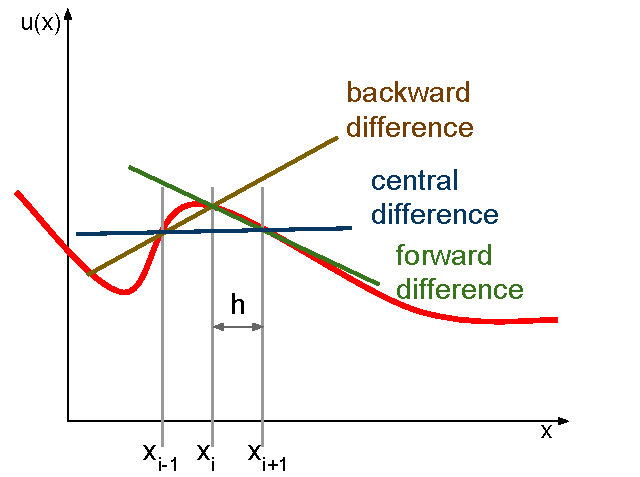
\includegraphics[width=0.7\textwidth]{chapters/chapter01/finite_differences.pdf}
	\caption{A one-dimensional representation of different kinds of finite differences around a point $x_i$}
	\label{fig:finite_differences}
\end{figure}

For the one-dimensional case, these finite differences are defined in the following way:
\begin{itemize}
\item Forward difference:
\begin{align}
\partial ^+ u(x) = \frac{u(x_{i+1}) - u(x_i)}{h} = \frac{u_{i+1} - u_i}{h} \approx (\frac{\partial u}{\partial x})_i % with $h = x_{i+1}-x_{i} $
\end{align}
\item Backward difference: 
\begin{align}
\partial ^- u(x) = \frac{u(x_{i+1}) - u(x_i)}{h} = \frac{u_{i} - u_{i-1}}{h} \approx (\frac{\partial u}{\partial x})_i % with $h = x_{i}-x_{i-1}$
\end{align}
\item Central difference: 
\begin{align}
\partial ^0 u(x) = \frac{u(x_{i+1}) - u(x_i)}{2h} = \frac{u_{i+1} - u_{i-1}}{2h} \approx (\frac{\partial u}{\partial x})_i % with $h = x_{i+1}-x_{i-1}$
\end{align}
\end{itemize}



% ./configure --download-fblaslapack --with-debugging=1 --download-mpich --download-hypre --download-ml --download-superlu_dist --download-parmetis --download-metis --download-ptscotch
We can see the difference between the finite difference and the exact solution $\mathlarger{(\frac{\partial u}{\partial x})_i}$ by taking a look at the Taylor series of the exact solution \cite{langer}:

\begin{itemize}
\item Forward difference: 
\begin{align}
\Big(\frac{\partial u}{\partial x}\Big)_i =  \frac{u_{i+1}-u_i}{h} - \frac{h}{2} \cdot \Big (\frac{\partial^2 u}{\partial x^2}\Big)_i + \hdots
\end{align}
\item Backward difference: 
\begin{equation}
\Big(\frac{\partial u}{\partial x}\Big)_i =  \frac{u_{i}-u_{i-1}}{h} + \frac{h}{2} \cdot \Big (\frac{\partial ^2 u}{\partial x^2}\Big)_i + \hdots
\end{equation}
\item Central difference: 
\begin{equation}
\Big(\frac{\partial u}{\partial x}\Big)_i =  \frac{u_{i+1} - u_{i-1}}{2h} - \frac{h^2}{6} \cdot \Big (\frac{\partial^3 u}{\partial x^3}\Big )_i + \hdots
\end{equation}
\end{itemize}

As one can see, for the difference between the exact solution and the finite difference there are $O(h)$ terms for the forward and the backward difference, while only $O(h^2)$ and higher order terms exist for the central difference. Hence, the approximation is much better for the central difference, which will be used in the following. Since second derivatives of a function $u(x)$ are required for Poisson's equation, it is also necessary to know its approximation. For that, we take the first derivation of $u(x)$
\begin{equation}
 \Big(\frac{\partial u}{\partial x}\Big)_i = u_x(x) \approx    \frac{u_{i+1} - u_{i-1}}{2h}
\end{equation}
and differentiate it:
\begin{equation}
\Big(\frac{\partial^2 u}{\partial x^2}\Big)_i = u_{xx}(x) \approx   \frac{\big(\frac{\partial u}{x}\big)_{i+1}   -  \big(\frac{\partial u}{x}\big)_{i-1}  }{2h} = \frac{u_{i-2} - 2u_i + u_{i+2}}{(2h)^2} 
\end{equation}
Only every other point is used here ($\hdots, u_{i-2}, u_i, u_{i+2}, \hdots)$, which means that the resolution of the grid decreased by half. To avoid that, the distance between the points is just halved ($2h \rightarrow h)$: 
\begin{equation}
u_{xx}(x) \approx \frac{u_{i+1} - 2u_i + u_{i-1}}{h^2} 
\label{equ:uxx}
\end{equation}

Now this approximation of $u_{xx}$ can be used on a grid \cite{langer}. 

\subsection{Poisson's Equation on a Grid}
The points $(x,y)$ in $\Omega$ that are used for the finite differences are the points that lie on a grid $\Omega_h$ \cite{Trottenberg:2000:MUL:374106}. This grid is, for our purposes, square, two-dimensional and has equidistant points, with a distance $h = 1/N$ from one point to its neighbour. Here $N$ is the number of grid points in one direction, without counting the zero point, so there are $(N+1)^2$ points in total in $\Omega_h$. We also assume that we only operate within the unit square $\Omega = (0,1)^2 \subset \mathbb{R}^2$. Then Poisson's equation
\begin{equation}
L u(x,y) = -\nabla^2 u(x,y) = f(x,y), \textnormal{ with } (x,y) \in \Omega
\end{equation}
can be transformed into the discrete version
\begin{equation}
L_h u^{\Omega_h}_h(x,y) = -\nabla^2_h u^{\Omega_h}_h (x,y) = f^{\Omega_h}_h(x,y), \textnormal{ with } (x,y) \in \Omega_h
\end{equation}
or, in a simpler notation
\begin{equation}
L_h u_{i,j} = -\nabla^2_h u_{i,j} = f_{i,j}.
\end{equation}


In order to solve this equation, it is necessary to know the boundaries $u_{0,j}, u_{i,0}, u_{N,j}, u_{i, N}$ with $0 \leq i,j \leq N$.
With the approximation for $u_{xx}(x)$ and $u_h (x_i,y_i) = u_{i,j}$ it is now possible to apply the approximated Laplace operator on $u_{i,j}$:

\begin{align}
\nabla^2 u(x,y) \approx \nabla^2_h u_{i,j}   &= \frac{\partial^2 u_{i,j} }{\partial x^2} + \frac{\partial^2 u_{i,j} }{\partial y^2} \nonumber \\
                      &= \frac{u_{i+h,j} - 2 u_{i,j} + u_{i-h,j} }{h^2} + \frac{u_{i,j+h} - 2 u_{i,j} + u_{i,j-h} }{h^2}\\
                      &= \frac{u_{i+h,j} + u_{i-h,j} - 4 u_{i,j} + u_{i,j+h} + u_{i,j-h} }{h^2} \nonumber
\end{align}
Now the Poisson equation on a two-dimensional grid can be written as
\begin{align}
-\nabla^2_h u_{i,j} = \frac{1}{h^2} (4 u_{i,j} -u_{i+h,j} - u_{i-h,j}  - u_{i,j+h} - u_{i,j-h} ) = f_{i,j}.
\end{align}
Here the stencil notation comes in handy \cite{Trottenberg:2000:MUL:374106}:
\begin{align}
-\nabla^2_h u_{i,j} = \frac{1}{h^2} 
\begin{bmatrix}
& -1 & \\
-1 & ~4 & -1 \\
& -1 & \\
\end{bmatrix}_h u_{i,j}
= f_{i,j}.
\label{equ:dis_poisson}
\end{align}

This equation shows that in our approximation, five unknown values $u_{i-1,j},$ $u_{i+1,j},$ $u_{i,j-1},$ $u_{i,j+1},$ $u_{i,j}$, depend on the function value $f_{i,j}$. In Fig.~\ref{fig:nat_order}, this means $f_{i,j}$ (in the middle of the 5-point stencil) determines the four adjacent u values and $u_{i,j}$.

\begin{figure}[tbp]
	\centering
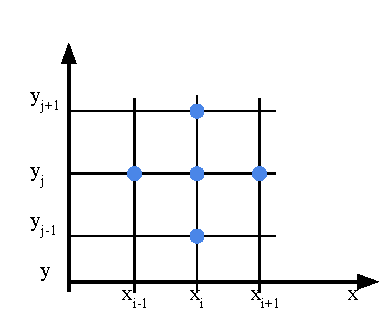
\includegraphics[width=0.42\textwidth]{chapters/chapter01/linear_order.pdf}
	\caption{A function value $f_{i,j}$ (in the middle of the 5-point stencil) determines the values of the unknowns $u_{i-1,j}, u_{i+1,j}, u_{i,j-1}, u_{i,j+1}, \textrm{ and } u_{i,j}$. }
	\label{fig:nat_order}
\end{figure}

\subsubsection*{Different Orderings}
The solution $u$ and the function $f$ both lie on a two-dimensional grid. However, it is  necessary to arrange them as one-dimensional vectors in order to bring the system to the form $Au = b$. One way to arrange these vectors is to use lexicographical ordering, so $u$ and $f$ are arranged as
\begin{align}
u &= [u_{0,0}, u_{1,0}, \hdots, u_{N,0}, u_{0,1}, u_{1,1}, \hdots, u_{N,1}, \hdots, u_{N,N} ]^T, \textrm{ and} \label{equ:natorder} \\
f &= [f_{0,0}, f_{1,0}, \hdots, f_{N,0}, f_{0,1}, f_{1,1}, \hdots, f_{N,1}, \hdots, f_{N,N} ]^T. \nonumber
\end{align}
An example of that  on a $4\times 4$ grid can be seen in Fig.~\ref{fig:nat_order_lexi_rb} a). Another kind of ordering the grid points is the red-black ordering (Fig.~\ref{fig:nat_order_lexi_rb}b), which has different properties in the possible degree of parallelization and yields a very different matrix $A$ \cite{Trottenberg:2000:MUL:374106}.


\begin{figure}[tbp]
	\centering
	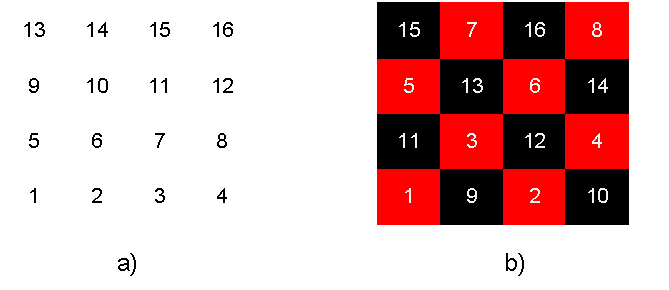
\includegraphics[width=0.65\textwidth]{chapters/chapter01/linear_order_lexi_rb.pdf}
	\caption{\textbf{a)} The points $x_{i,j}$ are sorted in a lexicographical ordering as in Equ. (\ref{equ:natorder}) to form vectors $u$ and $f$. \textbf{b)} Grid points sorted in the red-black ordering.}
	\label{fig:nat_order_lexi_rb}
\end{figure}

\subsubsection*{Combining it all to a linear system}
Now the example from Fig.~\ref{fig:nat_order_2} is useful: Given a two-dimensional grid with $N = 3$ and $h = \frac{1}{N} = \frac{1}{3}$ and lexicographical ordering, we want to solve the Poisson equation. For that, we start with expressing $f_5$: With (\ref{equ:dis_poisson}) and lexicographical order we get 
\begin{equation}
f_5 = 4 \cdot 3^2 \cdot u_5 - 3^2 \cdot u_1 - 3^2 \cdot u_4  - 3^2 \cdot u_6 - 3^2 \cdot u_9
\end{equation}






\begin{figure}[tbp]
	\centering
	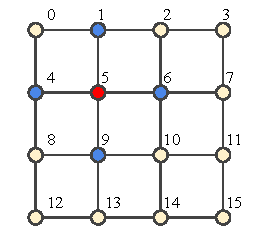
\includegraphics[width=0.5\textwidth]{chapters/chapter01/linear_order_2.pdf}
	\caption{Example of a grid with $h=\frac{1}{N} = \frac{1}{3}$. The points are sorted in a lexicographical order, so $f_5$ is a linear combination of $u_1, u_4, u_5, u_6 \textrm{ and } u_9$.}
	\label{fig:nat_order_2}
\end{figure}



By combining all points of the $4\times 4$ grid we obtain the linear system \cite{schwed}

\setcounter{MaxMatrixCols}{20}
\begin{equation}
\begin{bmatrix}
1  &    & &  &  &  & &  &  &  &  &  &  &   & &  \\
  &  1  & &  &  &  & &  &  &  &  &  &  &  & &  \\
  &     & 1 &  &  &  & &  &  &  &  &  &  &  & &  \\
  &     &  & 1 &  &  & &  &  &  &  &  &  &  & &  \\
  &     &  &  & 1 &  & &  &  &  &  &  &  &  & &  \\
  &  -9  &  &  & -9 &  36 & -9 &  &  & -9 &  &  &  &  & &  \\
  & &  -9  &  &  & -9 &  36 & -9 &  &  & -9 &  &  &  &  &   \\
  &     &  &  &  &  & & 1 &  &  &  &  &  &  & &  \\
  &     &  &  &  &  & &  & 1 &  &  &  &  &  & &  \\
  & & & & &  -9  &  &  & -9 &  36 & -9 &  &  & -9 &  &  &     \\
  & & & & & & -9  &  &  & -9 &  36 & -9 &  &  & -9 &  &       \\
  &     &  &  &  &  & &  &  &  &  & 1 &  &  & &  \\
  &     &  &  &  &  & &  &  &  &  &  & 1 &  & &  \\
  &     &  &  &  &  & &  &  &  &  &  &  & 1 & &  \\
  &     &  &  &  &  & &  &  &  &  &  &  &  & 1 &  \\
  &     &  &  &  &  & &  &  &  &  &  &  &  & & 1 \\
\end{bmatrix} 
\begin{bmatrix}
  u_{0}   \\
  u_{1}   \\
  u_{2}   \\
  u_{3}   \\
  u_{4}   \\
  u_{5}   \\
  u_{6}   \\
  u_{7}   \\
  u_{8}   \\
  u_{9}   \\
  u_{10}   \\
  u_{11}   \\
  u_{12}   \\
  u_{13}   \\
  u_{14}   \\
  u_{15}   \\
 \end{bmatrix} =
 \begin{bmatrix}
  f_{0}   \\
  f_{1}   \\
  f_{2}   \\
  f_{3}   \\
  f_{4}   \\
  f_{5}   \\
  f_{6}   \\
  f_{7}   \\
  f_{8}   \\
  f_{9}   \\
  f_{10}   \\
  f_{11}   \\
  f_{12}   \\
  f_{13}   \\
  f_{14}   \\
  f_{15}   \\
 \end{bmatrix}
 \label{equ:hugeA}
\end{equation}
Here, the ones in the matrix represent the fact that the boundary values $u_i = f_i$ are already known and only the rows corresponding to inner grid points show more than one non-zero. To be exact, they always have five non-zeros when using Equation~(\ref{fig:nat_order_2}), so a big linear system employs matrices where only a tiny percentage of elements is non-zero. We keep that thought in mind for later, when storing these matrices is discussed.


In more general situations, with a $(N+1) \times (N+1)$ grid, one gets a linear system
\begin{equation}
Au = f,
\end{equation}
by expressing all inner points of the grid and by taking care of boundary values. Here \textit{A} is a $(N+1) ^2 \times (N+1)^2$ matrix. This size originates from the fact that each of the $(N+1)^2$ function values $f_{i,j}$ is expressed as a linear combination of $(N+1)^2$ unknowns $u_{ij}$, so every row corresponds to one grid point. Now it becomes apparent that a high number of grid points results in huge linear systems that can only be solved with efficient algorithms. Fortunately it is not necessary to store the whole matrix \textit{A}, the operations are rather performed grid point by grid point with matrix values $A_{i,j}$ that can be deduced during the computation through a simple scheme. Such schemes are now given for both lexicographical and red-black ordering.

If the Dirichlet boundary conditions are eliminated, i.e. the rows corresponding to boundary points are skipped for now (the ones in (\ref{equ:hugeA})) and if lexicographical ordering is used, the matrix \textit{A} arises as a block tridiagonal matrix
\begin{equation}
A = \begin{bmatrix}
~T & -I  & &\\
-I & ~T & -I & \\
& -I & ~T & -I \\
& & -I & ~T\\
\end{bmatrix},
\end{equation}
with 
\begin{equation}
I = \begin{bmatrix}
1& & &  \\
&1 & & \\
& & 1 & \\
& & & 1 \\
\end{bmatrix}, \textrm{~~~~~~and~~~~~~} T = 
\begin{bmatrix}
~4 & -1& &  \\
-1&~4 & -1& \\
& -1& ~4 & -1 \\
& &-1 & ~4 \\
\end{bmatrix}
\end{equation}

For multigrid solvers that run highly parallel, the red-black ordering (see Fig.~\ref{fig:nat_order_lexi_rb}b)) is more important than lexicographical ordering. For the red black ordering, the red unknowns are not considered at the same time as the black unknowns, but rather one after another. The resulting matrix \textit{A} is again a block matrix, but the colours are partly separated from each other. For this ordering, there is a block $A_{rr}$ that represents red points that are connected to other red points, a block $A_{bb}$ for black points connected to black points, and blocks $A_{rb}$ and $A_{br}$ for red points connected to black points and vice versa: 

\begin{equation}
A_h = 
\begin{bmatrix}
A_{rr} & A_{rb}\\
A_{br} & A_{bb}\\
\end{bmatrix}
\end{equation}
Since (\ref{equ:dis_poisson}) does not connect any points of the same colour to each other, the blocks $A_{rr}$ and $A_{bb}$ are diagonal matrices with diagonal elements $\frac{4}{h^2}$, so the diagonal elements of \textbf{A} are the same for lexicographical and red-black ordering. A connection from point $x$ to point $y$ implies a connection from $y$ to $x$, so  $A_{rb} = A_{br}^T$. The resulting block matrix $A_{rb}$ is then \cite{Trottenberg:2000:MUL:374106}
\begin{equation}
A_{rb} = \frac{1}{h^2} 
\begin{bmatrix}
-1 & ~0 & -1 & & & &  & \\
-1 & -1 & ~0 & -1 & & &   & \\
-1 & ~0 & -1 & -1 & -1 &   & \\
   & -1 & ~0 & -1 & ~0 & -1 &    \\
   
   & & -1 & ~0 & -1 & ~0 & -1     \\
   & & & -1 & -1 & -1 & ~0 & -1     \\
     & & & & -1 & ~0 & -1 & -1   \\
       & & & &  & -1 & ~0 & -1  \\
\end{bmatrix}
\end{equation}
 
There are different ways of how to deal with such a linear system, the most efficient ones will be discussed in the next section.

\section{Introduction to Linear Systems}
Big linear system of the form $Au = b$ are usually solved iteratively, with an approximate solution $u^{(k)}$ that converges to $u = A^{-1}b$ \cite{golub1996matrix}. There are various ways to solve such a linear system, with different efficiencies and different kinds of applications. Therefore, it is essential to pick the most appropriate solver method. For example, the banded version of Gaussian elimination, a direct solver, has a complexity of $O(N^2)$, with a total number of unknowns $N$, while iterative solvers like the Jacobi iteration or the Gauss-Seidel iteration both have complexities of $O(N^2 \log \epsilon)$, with a discretization accuracy $\epsilon$ \cite{Trottenberg:2000:MUL:374106}. 

On the other hand, multigrid solvers, which rely on iterative solvers like the Gauss-Seidel or the Jacobi method, and specialized Poisson solvers like the total reduction method have an optimal efficiency of $O(N)$. What makes the multigrid method so powerful is the fact that even though it is not specialized on any particular kind of problem, it has the same efficiency as highly specialized Poisson solvers \cite{Trottenberg:2000:MUL:374106}. Since iterative solvers like the Jacobi method or the Gauss-Seidel method are the backbone of multigrid solvers, they will be discussed in the following.



%\subsection{Introduction to Jacobi and Gauss-Seidel iterations}
The Jacobi method is the simplest iterative method for solving the $Au = b$ problem \cite{golub1996matrix}. The idea of solving it is very simple and natural. For example, a problem with three unknowns can be rewritten as
\begin{align}
u_1 = (b_1 - a_{12}u_2 - a_{13}u_3) \big/ a_{11},\nonumber \\
u_2 = (b_2 - a_{21}u_1 - a_{23}u_3) \big/ a_{22}, \\
u_3 = (b_3 - a_{31}u_1 - a_{32}u_2) \big/ a_{33},\nonumber
\end{align}
If $u^{(k-1)}$ is an approximation of $u$, then it is very natural to calculate a new approximation as 
\begin{align}
u_1^{(k)} = (b_1 - a_{12}u_2^{(k-1)} - a_{13}u_3^{(k-1)}) \big/ a_{11},\nonumber \\
u_2^{(k)} = (b_2 - a_{21}u_1^{(k-1)} - a_{23}u_3^{(k-1)}) \big/ a_{22}, \\
u_3^{(k)} = (b_3 - a_{31}u_1^{(k-1)} - a_{32}u_2^{(k-1)}) \big/ a_{33}.\nonumber
\end{align}
Of course, the diagonal elements must not be zero \cite{golub1996matrix}. This procedure can be generalized for  $n \times n$ matrices:

\noindent\hspace*{15mm}\textbf{for } $i = 1:n$
\begin{align}
\hspace*{-25mm} u_i^{(k)} = \Bigg ( b_i - \sum_{j = 1}^{i-1} a_{ij}u_j^{(k-1)} - \sum_{j = i+1}^{n} a_{ij}u_j^{(k-1)} \Bigg ) \Bigg / a_{ii}
\end{align}
\hspace*{15mm}\textbf{end}

However, when the $u_j^{(k-1)}$ values from the first sum are used in this equation, there already exist more recently updated, hence more accurate values $u_j^{(k)}$. If we always use the most recently updated approximation of $u_j$, the Jacobi iteration turns into the Gauss-Seidel iteration:

\noindent\hspace*{15mm}\textbf{for } $i = 1:n$
\begin{align}
\hspace*{-25mm} u_i^{(k)} = \Bigg ( b_i - \sum_{j = 1}^{i} a_{ij}u_j^{(k)} - \sum_{j = i+1}^{n} a_{ij} u_j^{(k-1)} \Bigg ) \Bigg / a_{ii}
\end{align}
\hspace*{15mm}\textbf{end}

We can also describe both iterations in terms of matrices \cite{golub1996matrix}. Then we split \textit{A} into three parts, a strictly lower triangular, a diagonal and a strictly upper triangular part:

\begin{equation}
L_A = 
\begin{bmatrix}
0 & 0 & 0 \\
a_{21} & 0 & \\
a_{31} & a_{32} & 0
\end{bmatrix}, D_A = 
\begin{bmatrix}
a_{11} & 0 & 0 \\
0 & a_{22} & \\
0 & 0 & a_{33}
\end{bmatrix}, U_A = 
\begin{bmatrix}
0 & a_{12} & a_{13} \\
0 & 0 & a_{23}\\
0 & 0 & 0
\end{bmatrix}.
\end{equation}

With such a separation of \textit{A}, the iterations can be written in the form
\begin{equation}
M u^{(k)} = N u^{(k-1)} + b.
\end{equation}

Then the Jacobi method \cite{golub1996matrix} can be written as
\begin{equation}
D_A u^{(k)} = -(L_A + U_A) u^{(k-1)} + b,
\end{equation}
and the Gauss-Seidel method as
\begin{equation}
(D_A + L_A) u^{(k)} = U_A u^{(k-1)} + b.
\end{equation}

In Chapter~2 we will discuss how such iterative solvers are part of the multigrid idea. For now, we take a look at the machines that are capable of solving such problems, even if they get really enormous in size.

%%%%%%%%%%%%%%%%%%%%%%%%%%%%%%%%%%%%%%%%%%%%%%%%%%%%%%%%%%%%%%%%%%%%%%%%%%%%%%%%%%%%%%%%%%%%%%%%%%%%%%%%%
%%%%%%%%%%%%%%%%%%%%%%%%%%%%%%%%%%%%%%%%%%%%%%%%%%%%%%%%%%%%%%%%%%%%%%%%%%%%%%%%%%%%%%%%%%%%%%%%%%%%%%%%%
%%%%%%%%%%%%%%%%%%%%%%%%%%%%%%%%%%%%%%%%%%%%%%%%%%%%%%%%%%%%%%%%%%%%%%%%%%%%%%%%%%%%%%%%%%%%%%%%%%%%%%%%%
%%%%%%%%%%%%%%%%%%%%%%%%%%%%%%%%%%%%%%%%%%%%%%%%%%%%%%%%%%%%%%%%%%%%%%%%%%%%%%%%%%%%%%%%%%%%%%%%%%%%%%%%%
%%%%%%%%%%%%%%%%%%%%%%%%%%%%%%%%%%%%%%%%%%%%%%%%%%%%%%%%%%%%%%%%%%%%%%%%%%%%%%%%%%%%%%%%%%%%%%%%%%%%%%%%%
%%%%%%%%%%%%%%%%%%%%%%%%%%%%%%%%%%%%%%%%%%%%%%%%%%%%%%%%%%%%%%%%%%%%%%%%%%%%%%%%%%%%%%%%%%%%%%%%%%%%%%%%%


\section{Supercomputers}

After this introduction to mathematics and physics treated in this thesis, an overview on supercomputer is given. So what is a supercomputer? They are computers with a very high level of performance compared to regular computers and they were introduced in the 1960s as highly tuned conventional designs that processed their programs sequentially. Shortly after the introduction of these supercomputers, machines with an increasing amount of parallelism (e.g. four processors) emerged. In the 1970s, machines that operated on arrays of data with specialized math units started to be developed. An example of such a vector machine is the Cray-1, the first supercomputer that implemented the vector processor design. It operated at 80 MHz and had a peak performance of 250~MFLOPS --- around $1/370,000$ of the currently fastest computer~\cite{russell1978cray,top500sunway}. The applications for supercomputers at that time were primarily weather forecasting and aerodynamic research~\cite{russell1978cray}. Such a Cray-1 supercomputer is shown in Fig.~\ref{fig:cray_1}.

\begin{figure}[tbp]
	\centering
	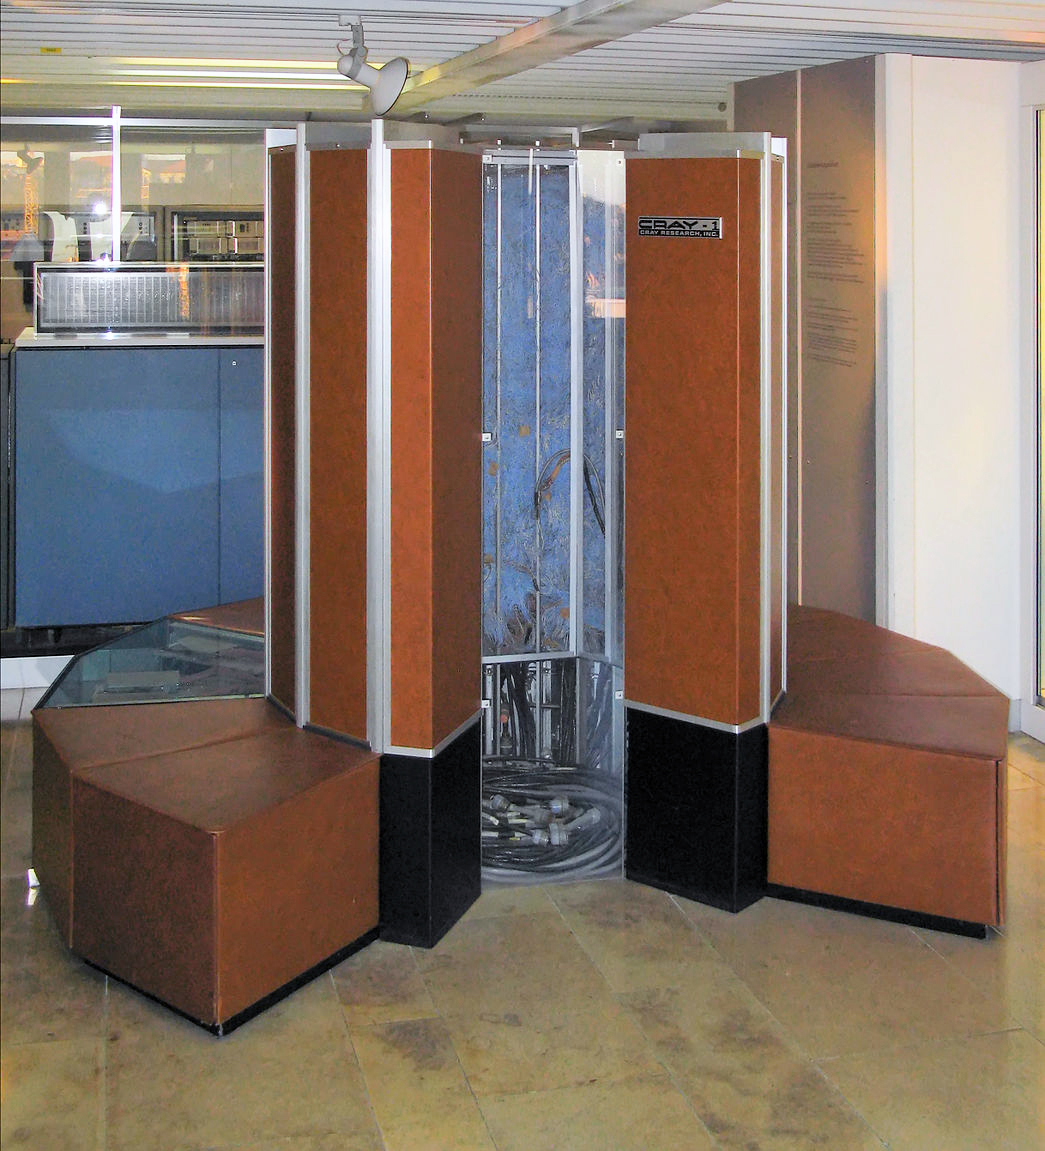
\includegraphics[width=0.5\textwidth]{chapters/chapter01/cray-1.jpg}
	\caption{The Cray-1 was the first supercomputer that implemented a vector processor design. It was first employed in 1976. Image by Wikimedia Commons \cite{wiki:cray_1_image}.} %https://commons.wikimedia.org/wiki/File:Cray-1-deutsches-museum.jpg
	\label{fig:cray_1}
\end{figure}

Vector machines were the dominating supercomputers for around two decades, until they gradually got replaced by machines that implemented massive parallelism by installing a huge number of off-the-shelf CPUs. 

\begin{figure}[tbp]
	\centering
	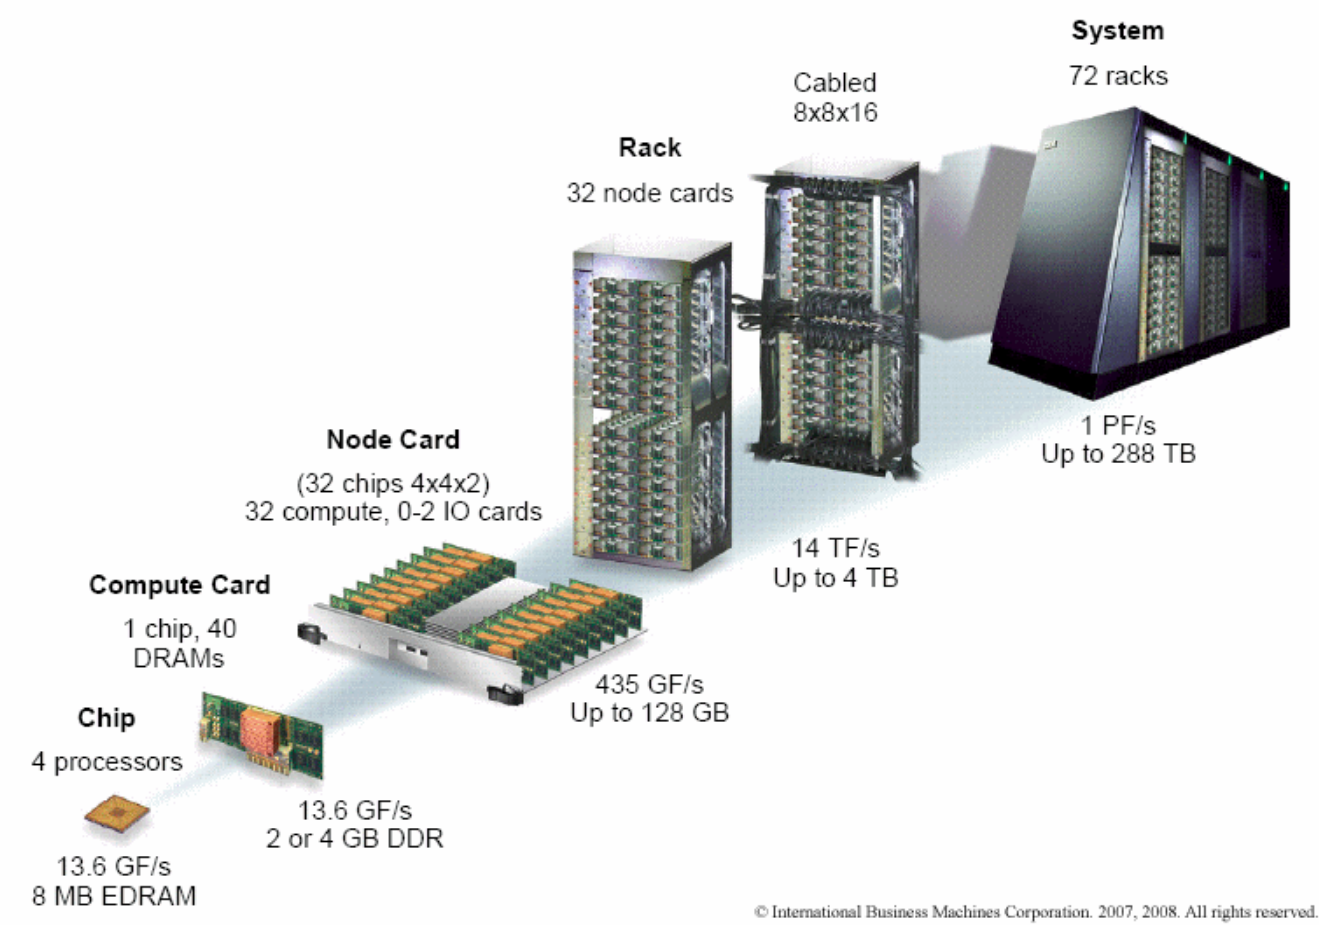
\includegraphics[width=0.8\textwidth]{architecture.png}
	\caption{Architecture of a supercomputer. Image by IBM \cite{image:supercomputer_arch}.} 
	\label{fig:finite_differences}
\end{figure}

Fig.~\ref{fig:finite_differences} shows a typical architecture of a modern supercomputer. Starting from the lowest level, there is a chip with a number of processor cores and multiple levels of cache memory. This cache can be dedicated to a single core or multiple cores. The chip is integrated on a compute card that combines the computing power of the processors with several gigabytes of main memory. Multiple compute cards (nodes) are combined on a node card, where the nodes are connected with some kind of interconnect. This interconnect has to provide a very high throughput and low latency, and can be implemented for example by using the InfiniBand standard \cite{liu2004high} or a multidimensional torus interconnect \cite{adiga2002overview}. The interconnect also connects racks with each other, so that, for example, 72 racks form a petaflop system with hundreds of terabytes of main memory.



Lately, also graphic processing units (GPUs) have been used in supercomputers. For example, the Titan supercomputer was upgraded from a CPU-only architecture to a hybrid-architecture that combines AMD Operton CPUs with NVIDIA Kepler GPUs. Through this upgrade, it increased its speed by a factor 10 and the power efficiency by a factor 5 \cite{titan}.


\subsection{Shared Memory vs Distributed Memory}

In early supercomputers with a small number of processors, data was shared among different processors by using a shared memory. An example for such a system is the Cray-1. If the memory is just one physical memory that is shared among all processors, the architecture is called uniform memory access (UMA) and the access times are similar for each processor. If the processors also use local memory, this local memory can be accessed much faster, so the architecture is called non-uniform memory access (NUMA). 

With a higher number of processors, however, it becomes increasingly difficult to manage such a shared architecture. Therefore, modern supercomputers with massive parallelism relinquish the shared memory idea and only use local memory. In this approach, a processor that needs non-local data has to request the data from other processors, which can be done for example with the message passing standard MPI \cite{mpi_forum}. When working with a system that uses distributed memory, it can be convenient to emulate a shared memory, i.e. there is a global memory space. This can be done with Partitioned Global Address Space (PGAS) languages like Unified Parallel C or Titanium (a scientific computing dialect of Java)~\cite{Yelick:2007:PPU:1278177.1278183}.


\subsection{Benchmarks}
In order to compare the performance of supercomputers, the TOP500 list of supercomputers is commonly used. This list is updated every six months and evaluates the number of floating point operations per second for the LINPACK benchmark \cite{linpack}. This benchmark generates a random dense linear system $Au = b$ in double precision arithmetic and solves it on distributed memory computers. However, the Linpack benchmark has been criticized for various reasons \cite{dongarra2007hpc}:
\begin{itemize}
\item The benchmark emphasizes the peak CPU performance and the number of CPUs. Other system properties, like local bandwidth and network bandwidth are neglected.
\item It ignores Amdahl's law, which attributes the time for non-parallelizable tasks. By using a fixed (big) problem size per processor, these non-parallelizable task can be neglected. However, for smaller problems than the benchmarked ones this might not be the case.
\item It returns only a single number to rate the system, which cannot reflect all properties adequately. On the other hand, a single number is needed for a list like the TOP500, which has made it attractive and popular over many decades.
\item It promotes the hype for more FLOPS, while other properties might be neglected by system designers.  
\end{itemize}

For the reasons stated above, other benchmarks have been developed. One of them is the High Performance Conjugate Gradient (HPCG) benchmark, a benchmark that tries to model data access patterns of real world problems such as sparse matrix multiplication. Since the memory bandwidth rather than the CPU limits the performance of the HPCG benchmark, the result in FLOPS is usually only a tiny fraction of the Linpack result \cite{dongarra2013toward}. For the HPCG benchmark the best result was obtained with the Japanese K computer with 0.603 PFLOPS, which is only 5.3\% of its Linpack performance \cite{HPCG}.


Another ranking is the Green500 list, which ranks the power efficiency of the systems in the TOP500 list. The systems are ordered by their GFLOPS/Watt while performing the Linpack benchmark. The list is topped by three Japanese supercomputers with a power efficiency of around 17 GFLOPS/Watt, which makes them almost three times more efficient than the number one of the TOP500 list. In general, the power efficiency of supercomputers has increased rapidly over the last few years and decades \cite{green500}. 


\subsection{Sunway TaihuLight}
As of May 2018, the number one on the TOP500 list of supercomputers is the Sunway TaihuLight, a truly enormous Chinese machine with a performance of 93~PFLOPS ($= 93\cdot 10^{15}$ floating point operations per second) for the Linpack benchmark~\cite{fu2016sunway}. This makes it three times more powerful than the former number one, which is now number two on the list  \cite{top500sunway}. 

The Sunway TaihuLight is used for four key domains of application:
\begin{itemize}
\item Climate, weather and earth system modelings,
\item Big data analytics,
\item Manufacturing applications (computational fluid dynamics (CFD), computer aided engineering (CAE)),
\item Life sciences
\end{itemize}

This system is not only extraordinary because of its performance, but also because it is ---~due to an US sanction~--- the first number one system that is completely based on Chinese processors. Each of the 40,960 nodes of the TaihuLight has a single 260-core processor with over 3 TFLOPS, so more than 10 million cores add up to a peak performance of around 125~PFLOPS. The processors that deliver this performance are ShenWei 64-bit RISC processors that run at a frequency of 1.45~GHz. However, the peak performance does not take memory transactions into account, so only 74\% of the peak performance are obtained with the Linpack benchmark, which is still a very respectable ratio. 

The High Performance Conjugate Gradient (HPCG) benchmark shows a weakness of the system: In this benchmark, only 0.3\% of the theoretical peak performance can be achieved, which is due to an imbalance between floating point power and memory performance. The memory controller delivers a bandwidth 136.5 GB/second for each socket. Compared to other supercomputers, this is only moderately high. Here, DDR3 memory is used, which is slower and needs more power than DDR4-memory. So with this relatively slow memory and a modest interconnect performance, the ratio of floating point operations per byte of data from memory is 22.4 FLOPS/byte (in double precision), a value that is far too high for many applications. Other processors have much lower ratios here, like Intel's Knights Landing processor with only 7.2 FLOPS/byte. On this system, each socket has a memory capacity of 32 GB, which adds up to 1.3~PB for the whole machine~\cite{fu2016sunway, dongarra2016report}.


What is also notable about the Sunway TaihuLight is its relatively low power consumption compared to other top ranked machines: It draws only 15.3~MW, while the number two on the TOP500-list draws 17.8MW for only a third of the performance. Such a power efficiency of 6.05 GFLOPS/Watt is a quite good result for a machine with that computing power, however it is far behind the number one of the Green500 which has an efficiency of 17.0 GFLOPS/Watt. It should be noted though that the top three positions in the Green500 list are in the bottom half of the TOP500 and they use a very different system architecture with 2048 cores per chip \cite{green500}.

The Sunway TaihuLight shows the big advances that China has made in high performance computing in the last few years: While there were no Chinese supercomputers in the TOP500 in 2001, there are 202 in the November 2017 list. It seems that China is well on track to reaching their goal of installing the first exascale ($10^{18}$ FLOPS) computer in 2020 \cite{dongarra2016report}.

\subsection{Vienna Scientific Cluster}
\label{sec:vsc3}

The Vienna Scientific Cluster (VSC) is a high performance computing system that is employed by several Austrian universities. There are two clusters available at the moment, VSC-2 and VSC-3; the latter was used for this project. It comprises 2020 computing nodes, each of them with two Intel Xeon E5-2650v2 eight-core-CPUs running at 2.6GHz and a total core count of 32768. Each node has 8~$\times$~8192~MB DDR3 memory, so the whole system has around 113~TB RAM.

With 596 TFLOPS the VSC-3 was ranked number 84 in the November 2014 TOP500 list, but now it is only on the rank 460.  As of April 2018, it is still the fastest supercomputer in Austria ~\cite{top500n_VSC3}. 

The VSC-3 uses around 540~kW of power, which has to be led away. For that, a new approach was picked: Instead of a conventional air cooling, the cores are submerged in 35 tons of paraffin oil, which transfers the heat away very efficiently due to its high heat conductivity. The oil, in turn, is cooled by water on the roof of the building and can reach up to 55°C~\cite{vsc_oil}.



%=========================================================